\section{Evaluation}

% \begin{frame}
%     \frametitle{Performance Overhead 2}
%     \centering
%     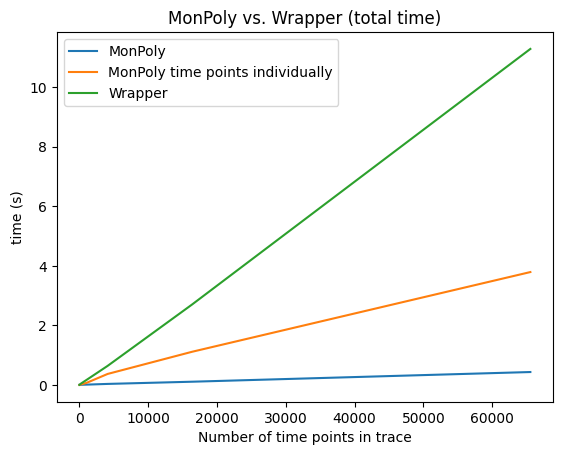
\includegraphics[width=0.9\linewidth]{diagrams/total-monpoly-vs-wrapper.png}
% \end{frame}

\subsection{Overhead of the Wrapper}
\begin{frame}{Overhead of the Wrapper}
    \begin{itemize}
        \item Random policy with intervals bounded by $[0,20)$
        \item Random trace with $4^i$ time points, for $i = 0,\dots,8$
        \item Measure the time it takes for MonPoly to monitor these traces
        \item Measure the time it takes for MonPoly to monitor the traces, when the time points are not in a single file, but sent individually
        \begin{itemize}
            \item This is a better simulation of online monitoring
        \end{itemize}
        \item Measure the time it takes for the wrapper to monitor these traces
        \item This was done \textbf{100 times} (with 100 different policies)
    \end{itemize}
\end{frame}

\begin{frame}{Overhead of the Wrapper}
    \centering
    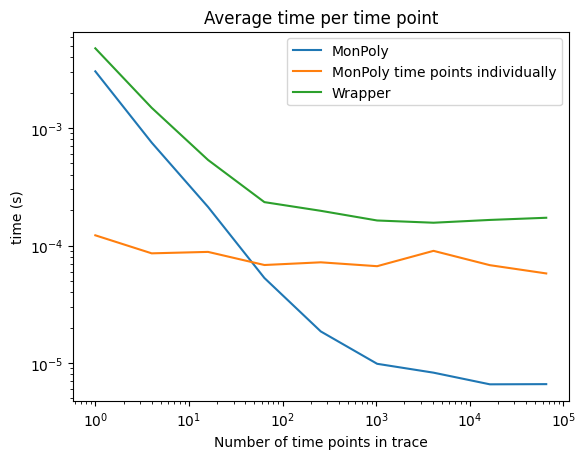
\includegraphics[width=0.9\linewidth]{diagrams/per-time-point-monpoly-vs-wrapper.png}
\end{frame}

\begin{frame}{Overhead of the Wrapper - Conclusion}
    \begin{itemize}
        \item More detailed profiling is required
        \item Possible sources of the overhead are:
        \begin{itemize}
            \item The conversion of our JSON format for logs to the MonPoly format
            \item The wrapper sends time points synchronously to MonPoly
            \item The wrapper must go over the events once to send them to MonPoly and again later to send them to QuestDB
        \end{itemize}
    \end{itemize}
    
\end{frame}


\subsection{Policy Change Optimization}
\begin{frame}{Policy Change Optimization}
    \begin{itemize}
        \item Policy change with 2 randomly generated formulas
        \item Intervals in policies are bounded by $[0,20)$.
        \item Random traces with $4^i$ time points, for $i = 0,\dots, 8$
        \item Load trace into wrapper and then initiate the policy change
        \item This was done 100 times, for 100 different policy pairs.
    \end{itemize}
\end{frame}

    
\begin{frame}{Policy Change Optimization}
    \centering
    % 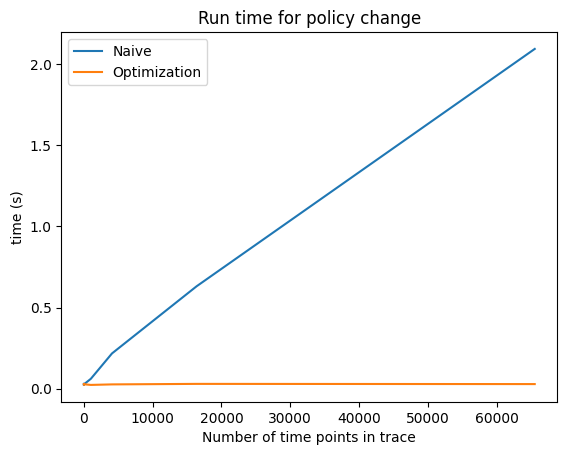
\includegraphics[width=0.5\linewidth]{diagrams/policy-change.png}
    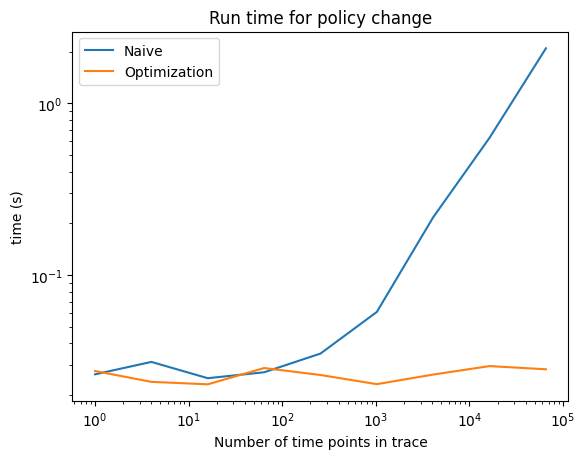
\includegraphics[width=0.9\linewidth]{diagrams/policy-change-log-log.png}
\end{frame}